\documentclass[12pt, titlepage]{article}

\usepackage{booktabs}
\usepackage{tabularx}
\usepackage{hyperref}
\usepackage{fancyhdr}
\usepackage{float}
\usepackage{subcaption}
\usepackage{graphicx}

\pagestyle{fancy}
\hypersetup{
    colorlinks,
    citecolor=black,
    filecolor=black,
    linkcolor=red,
    urlcolor=blue
}
\usepackage[round]{natbib}

\newcounter{tnum}
\newcommand{\tthetnum}{T\thetnum}
\newcommand{\tref}[1]{T\ref{#1}}

\title{SE 3XA3: Test Report\\Ultimate Tic Tac Toe}

\author{Team 3,
		\\ Kunal Shah - shahk24
		\\ Pareek Ravi - ravip2
}

\date{\today}

%% Comments

\usepackage{color}

\newif\ifcomments\commentstrue

\ifcomments
\newcommand{\authornote}[3]{\textcolor{#1}{[#3 ---#2]}}
\newcommand{\todo}[1]{\textcolor{red}{[TODO: #1]}}
\else
\newcommand{\authornote}[3]{}
\newcommand{\todo}[1]{}
\fi

\newcommand{\wss}[1]{\authornote{blue}{SS}{#1}}
\newcommand{\ds}[1]{\authornote{red}{DS}{#1}}
\newcommand{\mj}[1]{\authornote{red}{MSN}{#1}}
\newcommand{\mh}[1]{\authornote{red}{MH}{#1}}
\newcommand{\cm}[1]{\authornote{red}{CM}{#1}}


% team members should be added for each team, like the following
% all comments left by the TAs or the instructor should be addressed
% by a corresponding comment from the Team

\newcommand{\tm}[1]{\authornote{magenta}{Team}{#1}}


\begin{document}

\lhead{Team 3 - Test Report}
\rhead{Ultimate Tic Tac Toe}

\maketitle

\pagenumbering{roman}
\tableofcontents
\listoftables
\listoffigures

\newpage
\begin{table}[hp]
\caption{\bf Revision History}
\begin{tabularx}{\textwidth}{p{3cm}p{2cm}X}
\toprule {\bf Date} & {\bf Version} & {\bf Notes}\\
\midrule
December 5 & 0.0 & Initial commit\\
December 6 & 0.2 & list of all tests\\

\bottomrule
\end{tabularx}
\end{table}

\newpage

\pagenumbering{arabic}

\section*{Abstract}
This document describes the results of all the testing done for Ultimate Tic Tac Toe.

\section*{List of Test}

This section provides an overview of the tests completed. Tests are summarized
in the following table \ref{TbTestList}. 

\refstepcounter{tnum}
\begin{table}[hp]
\caption{\textbf{Table of Tests}} \label{TbTestList}
\begin{tabularx}{\textwidth}{p{1cm}X}
\toprule
\textbf{id} & \textbf{Test} \\
\midrule

\tthetnum\refstepcounter{tnum} \label{test1} & Click should set random tile \\
\tthetnum\refstepcounter{tnum} \label{test2} & Win inner board \\
\tthetnum\refstepcounter{tnum} \label{test3} & Draw inner board (tie) \\
\tthetnum\refstepcounter{tnum} \label{test4} & Win the full game\\
\tthetnum\refstepcounter{tnum} \label{test5} & Draw the full game\\
\tthetnum\refstepcounter{tnum} \label{test6} & Play Again\\
\tthetnum\refstepcounter{tnum} \label{test7} & Return to Board\\
\tthetnum\refstepcounter{tnum} \label{test8} & Click on a cell that is already occupied \\

\bottomrule
\end{tabularx}
\end{table}

\section{Functional Requirements Evaluation}
\subsubsection{User Input}

\begin{enumerate}

\item{in-test-id1\\}
\textbf {Testing if user's input being received}
					
Initial State: It is the start of a new game and the board is empty
					
Input: A click on any random cell of any inner tic tac toe board
					
Expected Output: That cell should have the user's character on it

Actual Output: The cell contains that user's character

Result: The test passed
					
\item{in-test-id2\\}
\textbf{Testing if user click on invalid inner board}
					
Initial State: Opponent has played on a inner board and it is the user's turn

Input: Click on a tile that they are not designated to click based on the
rules of the game
					
Expected Output: The board should not change at all. The game data should not change
and it is still the user's turn

Actual Output: Nothing happens

Resut: The test passed

\item{in-test-id3\\}
\textbf{Testing if user's input on cell already clicked}
					
Initial State: Opponent has played on a inner board and it is the user's turn
					
Input: Click on a tile that has already been clicked previously
					
Output: The board should not change at all. The game data should not change
and it is still the user's turn

\end{enumerate}

\subsubsection{Game Logic}

\begin{enumerate}

\item{log-test-id1\\}
\textbf{Test if inner board gets completed}

Type: Functional, Dynamic, Automatic
					
Initial State: Inner board is almost completed by user. It is their turn to
play in the inner board where they will complete it.
					
Input: Clicks on the cell that will complete the inner board
					
Output: The inner board will be marked with the character representing the
user
					
How test will be performed: This test will be performed automatically with the
use of the Karma Unit Test. The cell element will be clicked by the tester.
The logic will check if there is any three in a row in that inner board that
the player just played in. If there is a three in a row, the entire board is
deemed as completed and marked as so. The check for a three in a row is to
check all 8 possible win scenarios, i.e. three rows, three columns and two
diagonals

\item{log-test-id2\\}
\textbf{Test if inner board ends in draw}

Type: Functional, Dynamic, Automatic
					
Initial State: The board is in a state where an inner board only has 1 cell
available to click and it will result in that board being a draw

Input: Click on the only available cell
					
Output: The inner board will be marked with the character '-' meaning it is a
draw
					
How test will be performed: This test will be performed automatically with the
use of the Karma Unit Test. The cell element will be clicked by the tester.
The logic will check all 8 possible cases for a completed three in a row. If
non exist and the inner board is full it is classified as a draw.

\item{log-test-id3\\}
\textbf{Test if next move can be made on any incomplete inner board}

Type: Functional, Dynamic, Automatic
					
Initial State: Game board is partially filled with one inner board completed

Input: Click at a cell corresponding to a completed inner board
					
Output: All incomplete inner boards active
					
How test will be performed: When the click is made on the inner board, the
background of all inner boards that are not completed is set to blue. Based on
the array which contains a map of the board, a loop through all the inner
board elements and check their background colors. Any inner board that is not
complete will have a background style blue.

\item{log-test-id4\\}
\textbf{Test if user turns are alternating}

Type: Functional, Dynamic, Automatic
					
Initial State: Player with character O just made a move

Input: Click at any available cell
					
Output: The character changes to X
					
How test will be performed: When a click is made, the character should change
and the innerHTML should represent the other one.

\end{enumerate}

\subsubsection{Game Logistics}

\begin{enumerate}

\item{logistic-test-id1\\}
\textbf{Test if game launches}

Type: Functional, Dynamic, Manual
					
Initial State: User is in the file explorer
					
Input: User launches the html file in browser
					
Output: The game launches in all browsers and shows an empty UTTT game board.
					
How test will be performed: The user will launch the game from their file
explorer. If they are able to see a blank UTTT board, the game has launched.

\item{logistic-test-id2\\}
\textbf{Test if user input shows in window}

Type: Functional, Dynamic, Manual
					
Initial State: User has just opened game\\ %\textcolor{red}{Spelling - CM}
					
Input: User clicks on any cell
					
Output: Cell they clicked on should change appearance
					
How test will be performed: If the user's click was registered, it would
indicate that to the user by changing the cell they clicked on to the
character that represents them. This will be seen graphically.

\end{enumerate}
\section{Nonfunctional Requirements Evaluation}
Nonfunctional Requirements where tested using two methods, manual testing during the 
development of the game, and usability survey after revision 0 demonstration.
\subsection{Usability}
		
\subsection{Performance}

	
\section{Comparison to Existing Implementation}
This project is a reimplementation of the original Ultimate tic tac toe game ~\citep{githubREF}. Prior to starting this project we investigated the existing implementation. There were 3 main elements we wanted to change for our reimplementation of Ultimate Tic Tac Toe which can been seen in Figure~\ref{fig:Comparison}.
\begin{enumerate}
\item Rules explaining how to play the game
\item User interface (colours and ascetic)
\item Ability to repay the game
\end{enumerate}

\begin{figure}[H]
\begin{subfigure}{.5\textwidth}
  \centering
  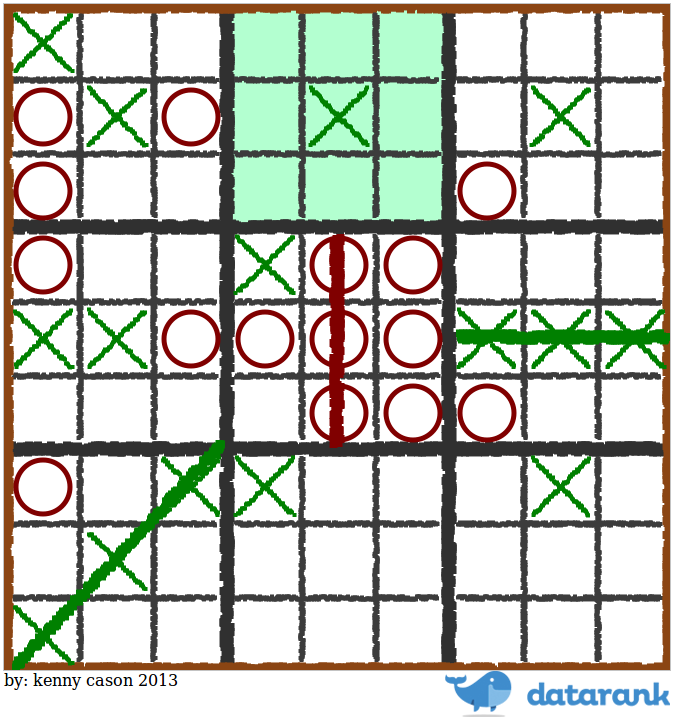
\includegraphics[width=0.95\linewidth]{../../ReferenceMaterial/SourceGame_screenshot.png}
  \caption{Original Game}
  \label{fig:sub1}
\end{subfigure}
\begin{subfigure}{.5\textwidth}
  \centering
  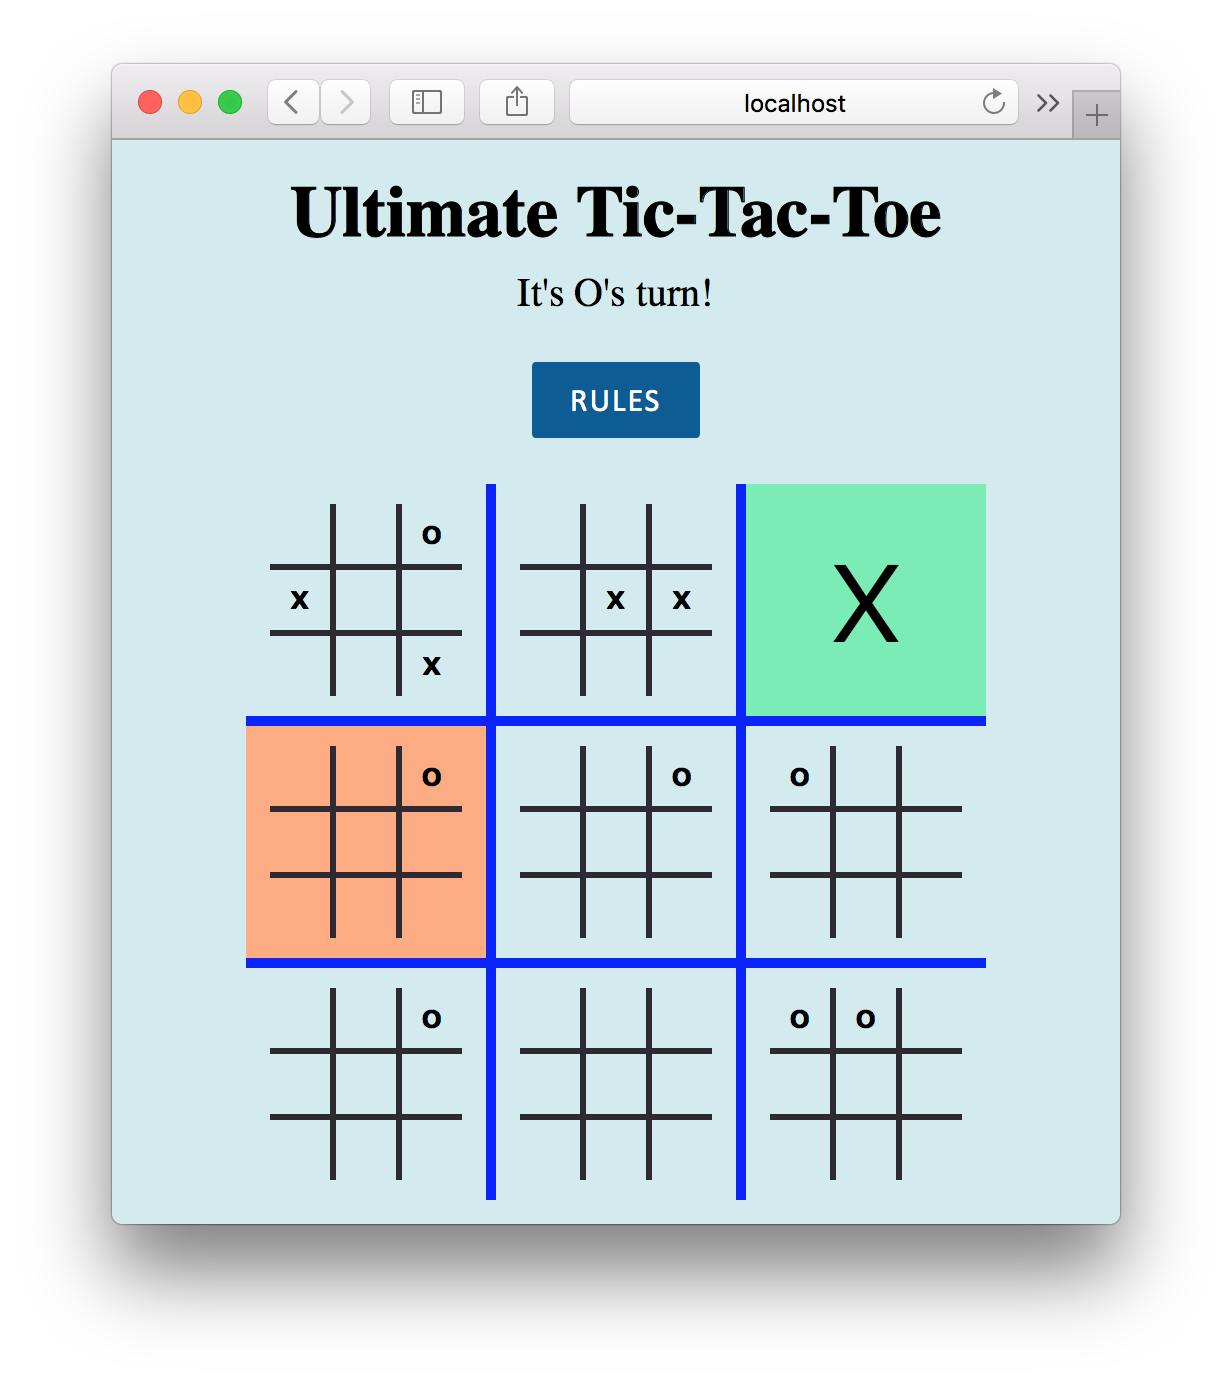
\includegraphics[width=1\linewidth]{../../ReferenceMaterial/XwinInnerBoard_screenshot.png}
  \caption{Reimplemented Game}
  \label{fig:sub2}
\end{subfigure}
\caption{Implementation Comparison}
\label{fig:Comparison}
\end{figure}

\section{Unit Testing}
\subsection{How to Test}
Unit testing was done using Karma and Jasmine frameworks. There is a folder called test
located in the src directory which contains the JavaScript file. In order to execute the testing framework, 
npm is required and all required packages are in a json file. Once all packages are installed, 
executing 'npm test' will run all the tests that are written in the test.js file.
\subsection{Tests}
The unit testing was done on the game logic which includes testing click functionality and some additional functionality such as the dropdown menus.
\section{Changes Due to Testing}
After performing unit testing on multiple browsers i.e.(Google Chrome, Safari, Firefox, Opera),
it was apparent that the game would not work on Firefox. The surveys also indicated that the game did
not work in Firefox. This was the only browser that was having issues with this. Unfortunately,
the reason for the incompatibility with Firefox is due to a click listener thus it could not be fixed. From
surveys, it was made clear that there was a scaling issue when playing on smaller displays, as such
changes were made to accommodate smaller devices screen sizes. The game board would adjust 
accordingly to the size of the display. 
\section{Automated Testing}
The automated testing was implemented with the Karma framework. This involved forcing Karma
to various game states and verifying if the results matched what was expected. The various 
states were a game ending in a win and ending in a draw.
\section{Trace to Requirements}
		
\section{Trace to Modules}		

\section{Code Coverage Metrics}

\bibliographystyle{plainnat}

\bibliography{TestReport}

\end{document}